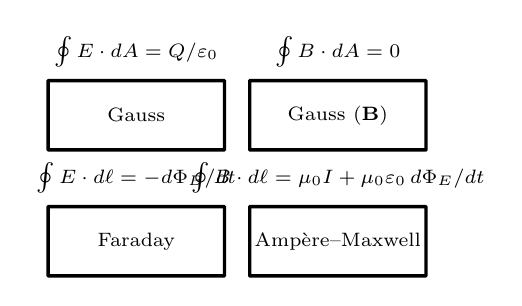
\begin{tikzpicture}[scale=0.8,font=\scriptsize]
\foreach \x/\y/\t in {-2.6/0.8/Gauss, 0.6/0.8/{Gauss ($\mathbf B$)}, -2.6/-1.2/Faraday, 0.6/-1.2/{Amp\`ere--Maxwell}}{
\draw[very thick,rounded corners=0.2] (\x-1.4,\y-0.55) rectangle (\x+1.4,\y+0.55);
\node[align=center] at (\x,\y) {\t};}
\node[align=left] at (-2.6,1.8) {$\oint E\cdot dA=Q/\varepsilon_0$};
\node[align=left] at (0.6,1.8) {$\oint B\cdot dA=0$};
\node[align=left] at (-2.6,-0.2) {$\oint E\cdot d\ell=-d\Phi_B/dt$};
\node[align=left] at (0.6,-0.2) {$\oint B\cdot d\ell=\mu_0I+\mu_0\varepsilon_0\,d\Phi_E/dt$};
\end{tikzpicture}
